\section {Evaluation\\}

In this section, we conducted experiments to evaluate the performance of several different polling methods.

\subsection{Settings \\}

\subsubsection{Evaluation Metrics \\}
During the experiments, we used the following parameters to benchmark 
the performance of message notification mechanisms. These parameters help 
to characterize different kinds of context.

\begin{itemize}
    \item {\bf Number of concurrent connections}: This variable allows us 
         to evaluate the scalability of different methods.
    \item {\bf Publish Interval}: This variable controls the frequency of 
         event publication by the server. 
    \item {\bf Polling interval}: This variable determines how long will 
        the method send a polling request to the server.
\end{itemize}

We used the following metrics to evaluate the performance of different
methods.
\begin{itemize}
    \item {\bf Network Traffic (NT)}: NT evaluates the network usage for
        different event notification methods.
    \item {\bf Mean Publish Trip time (MPT)}: The publish trip-time is 
        the time elapsed between the creation of a data by the server and 
        its reception by the client. It shows how long it takes for the 
        client to be updated when an event occurs.
    \item {\bf Received Message Percentage (RMP)}: RMP indicates the data 
        loss in during the network communication. 
    \item {\bf Server Memory Usage (SMU)}: In many real world long polling 
        system, the polling requests spent most of their time waiting for 
        the new events.[source needed] Thus, memory cost for each idle 
        polling requests is critical to the overall performance.
\end{itemize}

\subsubsection{Evaluation Environment \\}
The experiments are done in CMU's PEACE cluster. Each machine in the cluster has a 4 CPU cores(AMD Opteron Processor 4130, 2600 MHz, 512K cache size), 8 GB RAM and 1 physical 581 GB disk.

\subsection{Push Model vs. Poll Model\\}

* Design goal: Comparison between different models, what are the expected experimental results.

* How do you conduct the experiment?

* What is the exp results?

* Experiment analysis: What can you see from the experiment results? Does it match your expectation?

One of the biggest advantage of long polling is the significant reduction of frequently client polls.

In this section, we will conduct experiments to figure the network traffic incurred by three different strategies:

\subsection{Event vs. Thread\\}


\subsection{Extending PushUp Server}


\begin{itemize}
    \item {\bf client polling (CP): } Client will initiate an http request to the server polling for the latest updates on a regular basis (in the experiments we set the polling frequency to be 1 second).
    \item {\bf multithreading long polling(MLP): } Long polling based on multi threads. The server will created a thread for each incoming long polling request.
    \item {\bf event-based long polling(ELP): }Long polling based on event-based notification.
\end{itemize}

\begin{table}
\centering \caption{\label{tb:traffic} Network IO(Active Connection=10)}
\begin{tabular}{|l|l|l|l|l|l|}
    \hline  & 10 sec & 20 sec & 30 sec & 40 sec & 50 sec \\
    \hline CP & 12.7K & 25.8K & 39.8K & 55.2K & 68.2K \\
    \hline MLP & 1.27K & 1.27K & 1.27K & 1.27K & 1.27K \\
    \hline ELP & 1.27K & 1.27K & 1.27K & 1.27K & 1.27K \\
    \hline
\end{tabular}
\end{table}

\begin{table}
\centering \caption{\label{tb:traffic} Network IO(Active Connection=100)}
\begin{tabular}{|l|l|l|l|l|l|}
    \hline      & 10 sec & 20 sec & 30 sec & 40 sec & 50 sec \\
    \hline CP & 127.4K & 277.1K & 415.2K & 580.5K & 745.5K \\
    \hline MLP & 12.7K & 12.7K & 12.7K & 12.7K & 13.1K \\
    \hline ELP & 12.7K & 12.7K & 12.7K & 12.7K & 12.7K \\
    \hline
\end{tabular}
\end{table}

\begin{table}
\centering \caption{\label{tb:traffic} Network IO(Active Connection=1000)}
\begin{tabular}{|l|l|l|l|l|l|}
    \hline & 10 sec & 20 sec & 30 sec & 40 sec & 50 sec \\
    \hline CP & 1370.5K & 3457.1K & 5537.5K & 7282.5K & 10743.5K \\
    \hline MLP & 135.5K & 132.5K & 137.8K & 133.4K & 135.5K \\
    \hline ELP & 130.1K & 129.5K & 132.8K & 131.8K & 130.5K \\
    \hline
\end{tabular}
\end{table}

\begin{table}
\centering \caption{\label{tb:traffic} Network IO(Active Connection=1000)}
\begin{tabular}{|l|l|l|l|l|l|}
    \hline & 10 sec & 20 sec & 30 sec & 40 sec & 50 sec \\
    \hline CP & 0.6 sec & 0.7 sec & 0.5 sec & 0.7 sec & 0.8 sec \\
    \hline MLP & 0.1 sec & 0.0 sec & 0.1 sec & 0.2 sec & 0.1 sec \\
    \hline ELP & 0.2 sec & 0.1 sec & 0.1 sec & 0.4 sec & 0.2 sec \\
    \hline
\end{tabular}
\end{table}

\begin{table}
\centering \caption{\label{tb:traffic} Network IO(Active Connection=1000)}
\begin{tabular}{|l|l|l|l|l|l|}
    \hline & 10 sec & 20 sec & 30 sec & 40 sec & 50 sec \\
    \hline CP & 0.8 sec & 1.1 sec & 2.5 sec & 3.1 sec & 2.7 sec \\
    \hline MLP & 0.5 sec & 0.4 sec & 0.5 sec & 0.8 sec & 1.2 sec \\
    \hline ELP & 0.6 sec & 0.4 sec & 0.8 sec & 1.2 sec & 0.9 sec \\
    \hline
\end{tabular}
\end{table}

\begin{table}
\centering \caption{\label{tb:traffic} Network IO(Active Connection=1000)}
\begin{tabular}{|l|l|l|l|l|l|}
    \hline  & 10 sec & 20 sec & 30 sec & 40 sec & 50 sec \\
    \hline CP & 0.5 sec & 3.4 sec & 4.5 sec & 5.3 sec & 7.2 sec \\
    \hline MLP & 0.5 sec & 2.6 sec & 2.7 sec & 3.5 sec & 3.4 sec \\
    \hline ELP & 0.8 sec & 2.8 sec & 1.8 sec & 2.4 sec & 2.9 sec \\
    \hline
\end{tabular}
\end{table}

\begin{figure}[htb!]
\centering%
    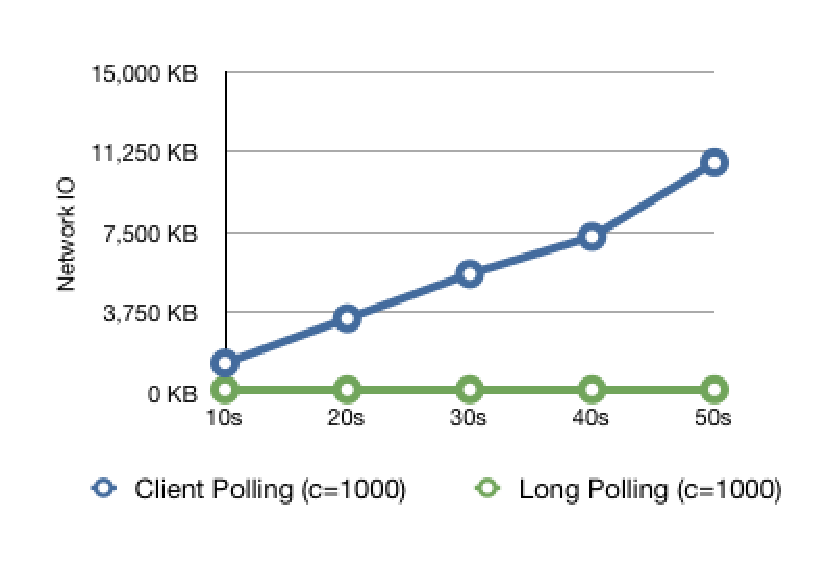
\includegraphics[scale=0.60]{figures/io.eps}
    \caption{Network traffic}
    \label{fig:traffic_io}
\end{figure}

\begin{figure}[htb!]
\centering%
    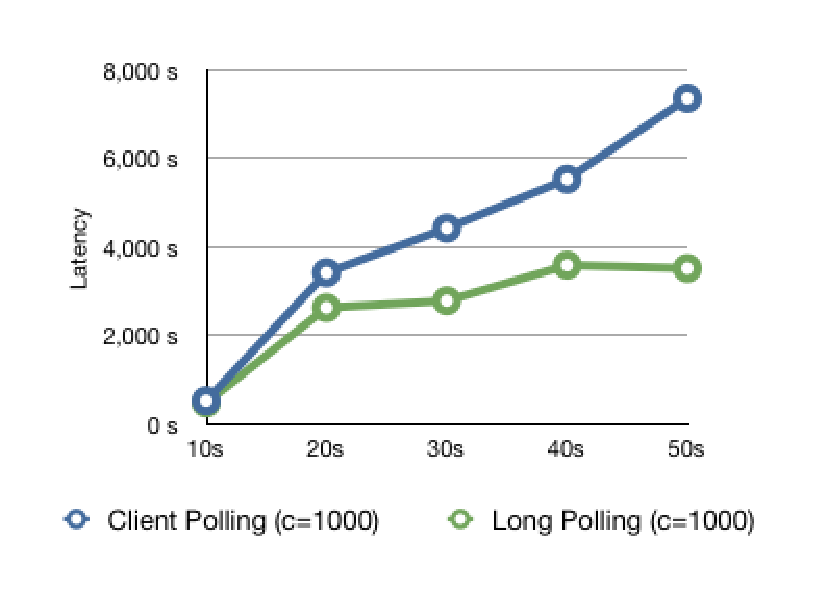
\includegraphics[scale=0.60]{figures/latency.eps}
    \caption{Latency}
    \label{fig:traffic_latency}
\end{figure}

\begin{figure}[htb!]
\centering%
    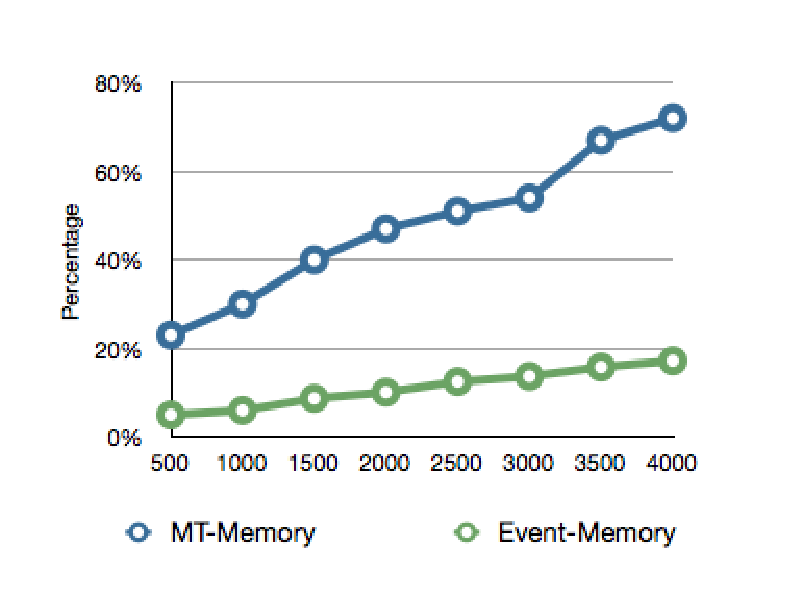
\includegraphics[scale=0.60]{figures/memory.eps}
    \caption{Comparison of the Memory Usage between Event-based and multithreading strategies}
    \label{fig:memory}
\end{figure}

\begin{figure}[htb!]
\centering%
    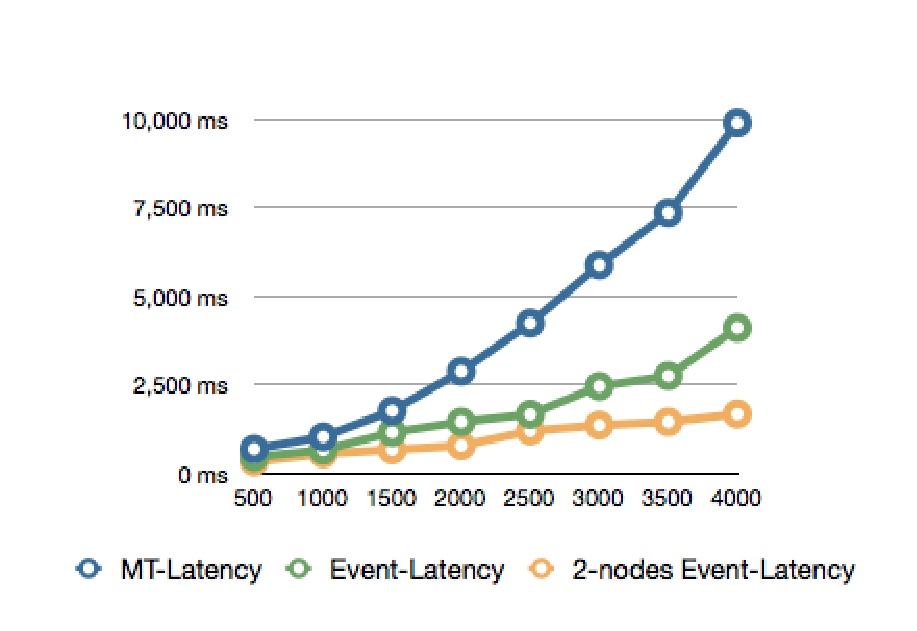
\includegraphics[scale=0.60]{figures/event_thread_latency.eps}
    \caption{Request Latency}
    \label{fig:memory}
\end{figure}

\subsection{Measuring the Active Connections\\}

